\chapter{HASIL DAN PEMBAHASAN}
\label{hasil-dan-pembahasan}
Bangunan yang dijadikan objek penelitian adalah \textit{climate chamber} DTNTF FT UGM. Dalam bab ini, akan dibahas mengenai hasil perancangan sistem kontrol sesuai dengan langkah-langkah yang dijelaskan pada Bab IV dengan memvariasikan berbagai macam masukan, kemudian mengetahui keluarannya. Variasi masukan dan keluaran akan dimodelkan dengan model jaringan saraf tiruan untuk mendapatkan parameter-parameter model yang dapat mengendalikan sistem bangunan.

\section{Pengembangan JST Plant}

Penulis menggunakan model JST yang telah dibangun oleh Tanto\cite{skripsiTanto} sebagai model acuan dalam penelitian ini. Model tersebut kemudian penulis kembangan kembali untuk mengingkatkan kinerjanya sebagai model \textit{plant}. \textit{Hyperparameter} yang digunakan Tanto pada pembangunan JST \textit{plant }ini dijelaskan pada tabel berikut:

\begin{table}[!h]
	\caption{Tabel Rancangan Model JST Plant Tanto}
	\label{tbl:5:NNPlantTanto}
	\centering
	% use packages: array
	\begin{tabular}{|p{5.7cm}|p{5cm}|}
		\hline
		\textbf{Nama Hyperparameter} & \textbf{Nilai Hyperparameter} \\ \hline
		Arsitektur & Feedforward Neural Network \\ \hline
		Pembagian Data & 50\% 25\% 25\% \\ \hline 
		Jumlah Layar Tersembunyi & 1 \\ \hline
		Jumlah Neuron pada Layar & [55] \\ \hline
		Fungsi Aktivasi Layar & Hyperbolic Tangent \\ \hline
		Algoritma Pembelajaran & Levenberg-Marquardt \\ \hline
		Mean Absolute Error & Td: 0,59$^\circ$C ; RH: 5,44\% \\ \hline
		Correlation Coefficient & Td: 96,23\% ; RH: 68,90\% \\ \hline
	\end{tabular}
\end{table}


\noindent \textbf{Variasi Pembagian Data} 

Dalam menentukan variasi pembagiaan data, penulis melakukan perbandingan dengan beberapa variasi pembagiaan data ke dalam 5 variasi. Kemudian, penulis membandingkan kinerja dari setiap pembagian data dengan menggunakan model JST dengan konfigurasi \textit{hyperparameter} sesuai rancangan penelitian sebelumnya\cite{skripsiTanto}.

\begin{table}[h!]
	\caption{Daftar variasi pembagian data}
	\label{tbl:5:DataSplitting}
	\centering
	% use packages: array
	\begin{tabular}{|p{3cm}|p{3cm}|p{1.5cm}|p{1cm}|p{1.5cm}|p{1cm}|}
		\hline
		Pembagian Data   & Persentase Data \\ \hline
		Data Splitting 0 & (50\% 25\% 25\%)\\ \hline
		Data Splitting 1 & (60\% 20\% 20\%)\\ \hline
		Data Splitting 2 & (70\% 15\% 15\%)\\ \hline
		Data Splitting 3 & (80\% 10\% 10\%)\\ \hline
		Data Splitting 4 & (80\% 15\% 05\%)\\ \hline
		Data Splitting 5 & (85\% 10\% 05\%)\\ \hline
	\end{tabular}
\end{table}

\begin{figure}[!h]
	\centering
	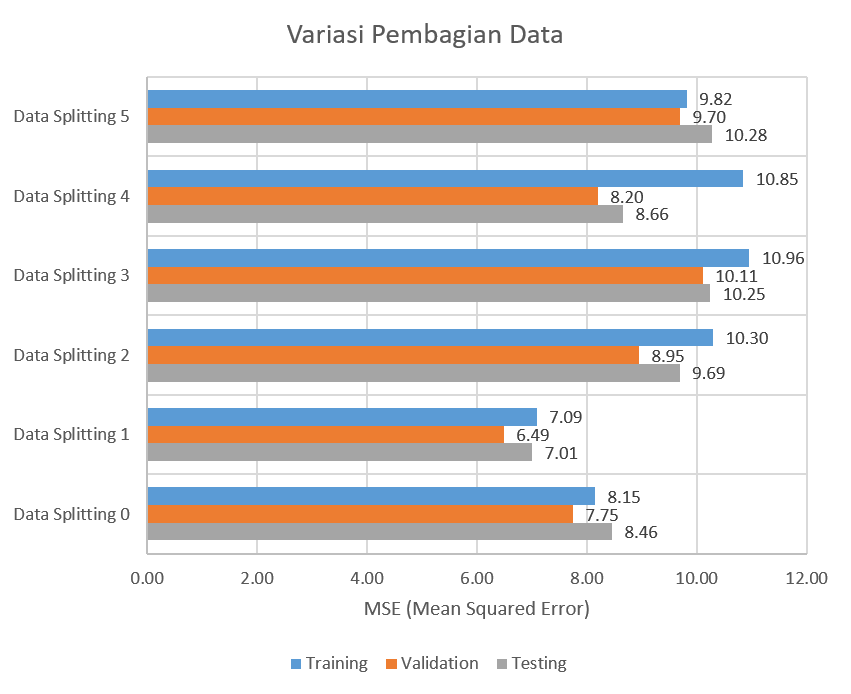
\includegraphics[width=0.9\textwidth]{figures/DataSplittingResult}
	\caption{}
	\label{fig:5:DataSplittingResult}
\end{figure}

Pada Tabel \ref{tbl:5:DataSplitting}, "Data Splitting 0" merupakan konfigurasi pembagian data yang digunakan oleh Tanto pada penelitian sebelumnya dalam membangun model JST \textit{plant}. Pada tabel yang penulis sajikan, penulis menulis pembagian data dengan format 'Data Splitting n' dan '(x\% y\% z\%)' dimana n = nomor variasi, x = pembagian data pelatihan, y = pembagian data validasi, dan z = pembagian data pengujian. \\

\begin{figure}[!h]
	\centering
	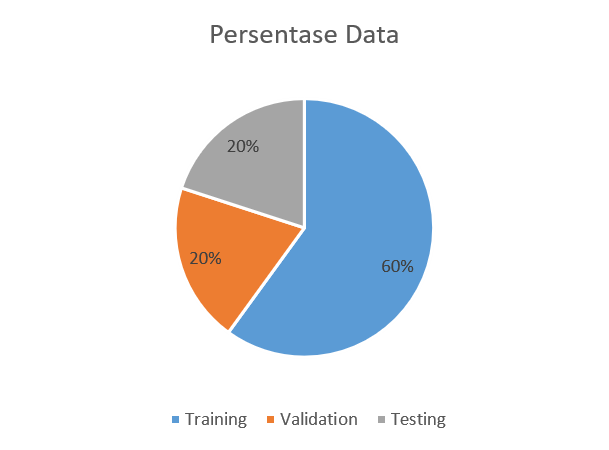
\includegraphics[width=1\textwidth]{figures/DataSplittingFinal}
	\caption{}
	\label{fig:5:DataSplittingFinal}
\end{figure}

Pembagian data terbaik yang penulis gunakan yaitu pembagian data bernama "Data Splitting 4". Data dibagi menjadi 3 bagian, yakni 80\% data pelatihan, 15\% data validasi, dan 5\% data pengujian.\\

\begin{table}[!h]
	\caption{Tabel Rancangan Model JST Plant Penulis}
	\label{tbl:5:NNPlantRidhan}
	\centering
	% use packages: array
	\begin{tabular}{|p{5.7cm}|p{5cm}|}
		\hline
		\textbf{Nama Hyperparameter} & \textbf{Nilai Hyperparameter} \\ \hline
		Arsitektur & Feedforward Neural Network \\ \hline
		Pembagian Data & 80\% 15\% 05\% \\ \hline 
		Jumlah Layar Tersembunyi & 1 \\ \hline
		Jumlah Neuron pada Layar & [55] \\ \hline
		Fungsi Aktivasi Layar & Hyperbolic Tangent \\ \hline
		Algoritma Pembelajaran & Levenberg-Marquardt \\ \hline
		Mean Absolute Error & Td: 0,57$^\circ$C ; RH: 5,40\% \\ \hline
		Correlation Coefficient & Td: 93,91\% ; RH: 72,05\% \\ \hline
	\end{tabular}
\end{table}


\section{Perancangan Sistem Kontrol JST}

\subsection{Perancangan JST Blok Kontroler}

\subsection{Perancangan Diagram Blok Sistem Kontrol}
